
\subsection{Description}
\begin{itemize}
    \item An Machine Readable Zone is composed of two lines of 44 characters
    \item Numbers and punctuations not authorized in the name field
    \item Hyphens are replaced by a filler character ('<')
    \item Apostrophes and commas are omitted
    \item First and last names are separated by 2 filler characters
    \item White characters are replaced by filler characters
\end{itemize}

\paragraph{Check Digits Calculation}
Check digits are computed for each protecfields. They are calculated modulo 10
with continous repetitive weihting of 731
\begin{itemize}
    \item Letters are mapped to their corresponding numerical value:
    A=10, B=11, \ldots,Z=35, '<' = 0.
    \item From left to right, each numerical value is multiplied by the weight
    appearing in the same sequential position.
    \item The product of each multiplication is added modulo 10
\end{itemize}
Ex: Calculate the check digit of the document number "EH123456<".
\begin{table}[ht!]
    \centering
    \begin{tabular}{c|c|c|c|c|c|c|c|c|c|}
        Number & E & H & 1 & 2 & 3 & 4 & 5 & 6 & < \\
        & 14 & 17 & 1 & 2 & 3 & 4 & 5 & 6 & 0 \\
        \hline
        Weight & 7 & 3 & 1 & 7 & 3 & 1 & 7 & 3 & 1\\
        \hline
        $N\times W \mod{10}$ & 98 & 51 & 1 & 14 & 9 & 4 & 35 & 18 & 0\\
    \end{tabular}
\end{table}
$$ 98+51+1+14+9+4+35+18 = 230 $$
$$ 230 \mod 10 = 0 $$
The remainder of the division is the check digit 0.

\subsubsection{Technical facts about the passport}
\begin{itemize}
    \item Tag is passive, i.e no internal battery
    \item Tag has a microprocessor (public-key crypto)
    \item Official distance 10cm
    \item EEPROM capacity: 32KB (minimum)
\end{itemize}

\subsubsection{Passport Content}
\begin{itemize}
    \item UID is publicly available
    \item Publicly available data, possibly after authentication
    \begin{itemize}
        \item Some data groups (DG)
        \item List of data groups on the considered passport (COM)
        \item Cryptographic material signature and hashes (SOD)
    \end{itemize}
    \item Data never supplied by the tag
    \begin{itemize}
        \item Two symmetric key $K_{ENC},K_{MAC}$ (can be retrieved from MRZ)
        \item One private key $K_{pr}$ (protected memory)
    \end{itemize}
\end{itemize}

\subsection{Protection Mechanisms}
\begin{figure}[ht!]
    \centering
    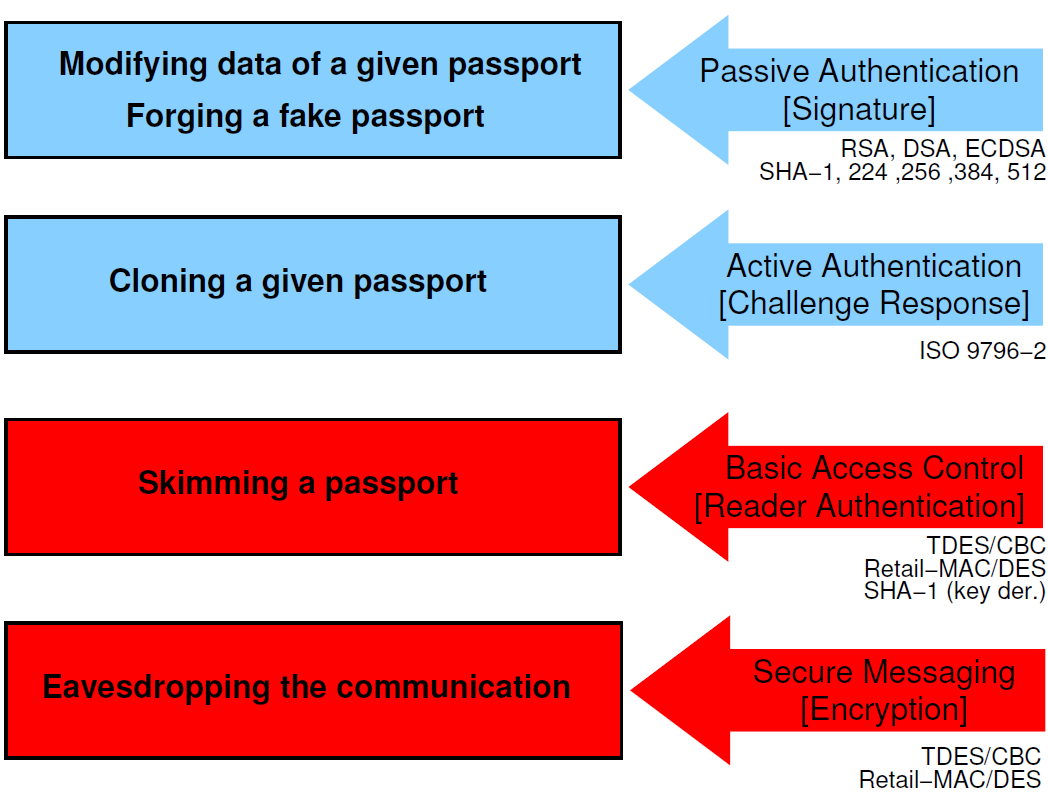
\includegraphics[scale=0.5]{img/e-passport}
\end{figure}

\subsubsection{Passive Authentication}
\begin{figure}[ht!]
    \centering
    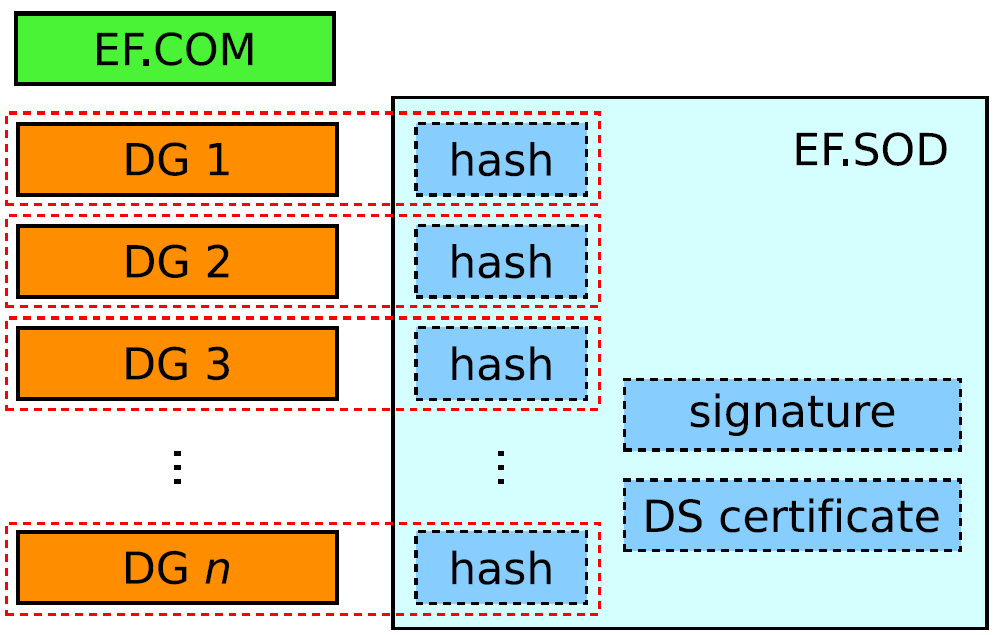
\includegraphics[scale=0.5]{img/passive-authentication}
\end{figure}

\begin{itemize}
    \item Passive authentication is a mandatory security mechanism, it proves
    that the file EF.SOD and LDS are authentic and not modified.
    \item EF.SOD contains the hash value of each present DG, and signature
    calculated by the issuing State over values.
    \item The signature can be checked using the Document Signer (DS) X.509
    certificate. (available from EF.SOD)
    \item The DS certificate can be checked using the Country Signing CA (CSCA)
    X.509 cerficate.
    \begin{itemize}
        \item The ICAO PKD does not publish the CSCA certificates
        \item CSCA certificates and revocation lists should be exchanged
        according to bilateral agreements
    \end{itemize}
\end{itemize}

\paragraph{Recommandations} According to DOC 9303:
\begin{itemize}
    \item The passive authentication should use RSA,DSA or ECDSA for the
    signature schemes
    \item SHA-1,SHA-2 for the hash algorithm
    \item CSCA keys should be renewed every three to five years and the DS
    keys every three months
\end{itemize}

\subsubsection{Active Authentication}
%%TODO add skecth
\begin{itemize}
    \item The active authentication is an optional security mechanism
    \item Aim is to prove the EF.SOD belongs to the authentic ePassport, i.e
    it is not a cloned one
    \item Two-pass CR protocol ISO 9796i\text{-}2 Digital Signature Scheme 1
    \item ePassport's public key is stored in DG15
\end{itemize}

The active authentication should rely on RSA,DSA or ECDSA and minimum sizes for
the security parameters should be 1024 bits, 1024 and 160 bits, and 160 bits,
respectively.
%%TODO example wih RSA/SHA1

\subsubsection{Access Control and Secure Messaging}
\begin{figure}[ht!]
    \centering
    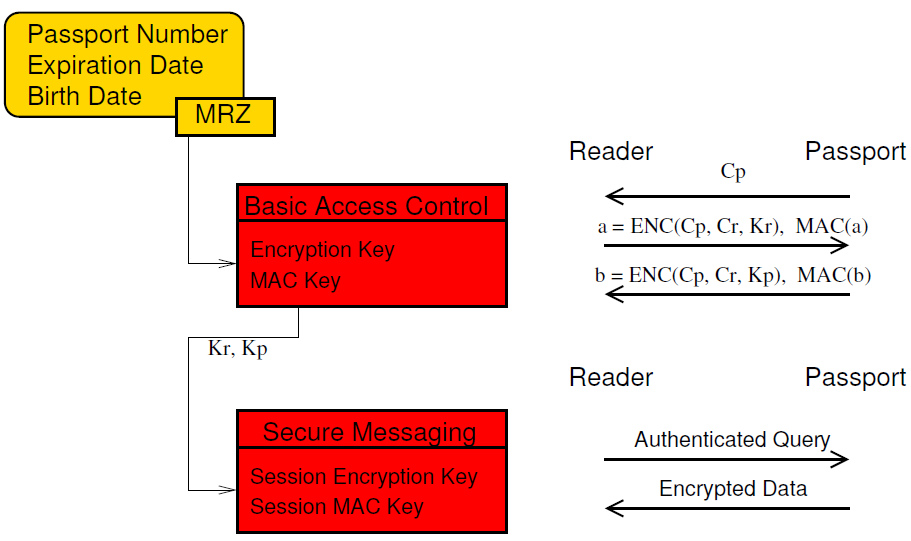
\includegraphics[scale=0.5]{img/access-control}
\end{figure}
\begin{itemize}
    \item Three-pass CR protocol according to ISO 11770\text{-}2 Key Establishment
    Mechanism 6, 2-key 3DES as block cipher
    \item Nonces should be 8-byte long
    \item Encryption done using 3DES in CBC mode with zero-IV according to
    ISO 11568\text{-}2
    \item A cryptographic checksum is calculated over: ISO 9797\text{-}1 MAC
    Algorithm 3 (i.e Retail-MAC), based on DES, zero-IV, ISO 9797\text{-}1 Padding
    Method 2
    \item Encryption and MAC keys derived from the MRZ using SHA-1
\end{itemize}

\paragraph{Key Derivation}
\begin{enumerate}
    \item Set $ K_{seed} = trunc_{16}(SHA-1(MRZ\_info))\quad or\ (K_r \oplus K_p)$
    \item Set $ D = K_{seed}||00000001 $
    \item Compute $ H = SHA-1(D) $
    \item First 16 bytes of H are set to the 2-key 3DES $ K_{ENC} $
    \item Set $ D = K_{seed}||00000002 $
    \item Compute $ H = SHA-1(D) $
    \item First 16 bytes of H are set to the 2 DES keys $K_{MAC} $
    \item Adjust the parity bits of the DES keys
\end{enumerate}

\subsection{Weaknesses}
BAC keys are derived from the MRZ, especially date of birth, date of expiry,
passport number. But passport numbers are usually not random. DOB and DOE are
neither random.

\begin{itemize}
    \item Relay Attacks: Passport is based on ISO 14443, so it can require to
    increase the timeouts.
    \item Evidence of Presence: Abuse the active authentication which can be
    doable without passing the BAC
    \item Chain og Trust: If the root certificate cannot be verified, making a
    fake passport is quite easy
\end{itemize}
